% -*- TeX:de -*-
\NeedsTeXFormat{LaTeX2e}
\documentclass[12pt,a4paper]{article}
\usepackage[german]{babel} % german text
\usepackage[DIV12]{typearea} % size of printable area
\usepackage[T1]{fontenc} % font encoding
%\usepackage[latin1]{inputenc} % most likely on Windows
\usepackage[utf8]{inputenc} % probably on Linux
\usepackage{multicol}

% PLOTTING
\usepackage{pgfplots} 
\usepackage{pgfplotstable}
\usepackage{url}
\usepackage{graphicx} % to include images
\usepackage{tikz}
\usepackage{subfigure} % for creating subfigures
\usepackage{amsmath} % a bunch of symbols
\usepackage{amssymb} % even more symbols
\usepackage{booktabs} % pretty tables
\usepackage{makecell} % multi row table heading

% a floating environment for circuits
\usepackage{float}
\usepackage{caption}

%\newfloat{circuit}{tbph}{circuits}
%\floatname{circuit}{Schaltplan}

% a floating environment for diagrams
%\newfloat{diagram}{tbph}{diagrams}
%\floatname{diagram}{Diagramm}

\selectlanguage{german} % use german

\begin{document}

%%%%%%% DECKBLATT %%%%%%%
\thispagestyle{empty}
			\begin{center}
			\Large{Fakultät für Physik}\\
			\end{center}
\begin{verbatim}


\end{verbatim}
							%Eintrag des Wintersemesters
			\begin{center}
			\textbf{\LARGE SS 14}
			\end{center}
\begin{verbatim}


\end{verbatim}
			\begin{center}
			\textbf{\LARGE{Physikalisches Praktikum\\ für das Bachelorstudium}}
			\end{center}
\begin{verbatim}




\end{verbatim}

			\begin{center}
			\textbf{\LARGE{PROTOKOLL}}
			\end{center}
			
\begin{verbatim}

\end{verbatim}

			\begin{flushleft}
			\textbf{\Large{Experiment (Nr., Titel):}}\\
							%Experiment Nr. und Titel statt den Punkten eintragen
			\LARGE{PS05 Polarisation}	
			\end{flushleft}

\begin{verbatim}

\end{verbatim}	
							%Eintragen des Abgabedatums, oder des Erstelldatums des Protokolls
			\begin{flushleft}
			\textbf{\Large{Datum:}} \Large{13.3.2014}
			\end{flushleft}
			
\begin{verbatim}
\end{verbatim}
							%Namen der Protokollschreiber
		\begin{flushleft}
			\textbf{\Large{Namen:}} \Large{Patrick Braun, Johannes Kurz}
			\end{flushleft}

\begin{verbatim}


\end{verbatim}
							%Kurstag und Gruppennummer, zb. Fr/5
			\begin{flushleft}
			\textbf{\Large{Kurstag/Gruppe:}} \Large{DO/4}
			\end{flushleft}

\begin{verbatim}

\end{verbatim}
							%Name des Betreuers, das Praktikum betreute.
			\begin{flushleft}
			\LARGE{\textbf{Betreuer:}}	\Large{Erhard Schafler}	
			\end{flushleft}

%%%%%%% DECKBLATT ENDE %%%%%%%
\pagebreak
\setlength{\columnsep}{20pt}
\begin{multicols}{2}

%%%%%%%%%%%%%%%%%%%%%%%%%%%%%%%%%%%%%%%%%%%%%%%%

%\begin{figure}[H]
%	\centering
%	\includegraphics[scale=0.35]{./data/beugung.png}
%	\caption{Beugungsmuster Einzelspalt (echtes Foto; schwarz durch weiß ersetzt)}
%	\label{fig:beugungsmuster}
%\end{figure}


%\begin{figure}[H]
%	\centering
%	\pgfplotstabletypeset[
%			columns={abstand, n},
%			col sep=&,
%			columns/abstand/.style={precision=2, zerofill, column name=\makecell{$Abstand$\\$(\pm 0.05)[mm]$} }, 
%			columns/n/.style={column name=\makecell{$n$\\$(Ordnung)$}, precision=0},
%			every head row/.style={before row=\hline,after row=\hline\hline},
%			every last row/.style={after row=\hline},
%			every first column/.style={column type/.add={|}{} },
%			every last column/.style={column type/.add={}{|} }
%			]{
%			abstand & n
%			12.9 & 1
%			24.45 & 2
%			37.40 & 3
%			49.35& 4
%			62.45 & 5
%			74.45 & 6
%			87.45 & 7
%			100.25 & 8
%			
%			}
%	\caption{Messwerte Einzelspalt}
%	\label{tab:werte_einzelspalt}
%\end{figure}



%%%%%%%%%%%%%%%%%%%%%%%%%%%%%%%%%%%%%%%%%%%%%%%%
%%%%%%%%%%%%%%%%%%%%%%%%%%%%%%%%%%%%%%%%%%%%%%%%
\section{Grundlagen, Theorie und Versuchsaufbau}

\subsection{Brewster Winkel}
Durch die Eigenschaft von Licht, aus vertikalen und horizontalen Komponenten zu bestehen, wird bei einer Einstrahlung von Licht auf einen Körper (z.B. von Luft auf Glas) nur ein Teil reflektiert und zwar genau jener Anteil der senkrecht auf die Einfallsebene steht.\\
Ist Licht nur senkrecht zur Einfallsebene polarisiert, wird immer weniger Licht reflektiert, bis nur noch Hintergrundrauschen fest zu stellen ist. Dieses Rauschen stammt jedoch von Umgebungslicht oder thermischer Strahlung.\\ 
Der Winkel des eingestrahlten Lichtes, bei dem nicht mehr reflektiert wird, heißt Brewster Winkel.\\
Ein einfacher geometrischer Zusammenhang beschreibt wie folgt den Winkel:

$$tan(\alpha_B) = \frac{n_2}{n_1}$$

\noindent
Gemessen werden kann die Lichtintensität. Lichtintensität kann mit Hilfe eines Fotowiderstandes gemessen werden. Die Funktionsweise ist wie folgt: "Je höher der Lichteinfall, desto kleiner wird aufgrund des inneren fotoelektrischen Effekts sein elektrischer Widerstand." [2] Diesen Umstand werden wir später noch benötigen.\\
\\
Der Aufbau zur Messung des Winkels benötigt eine planparallele Platte einen Polarisator (Prisma, [1](p. 3)) und eine Fotodiode (siehe Diskussion). Der Aufbau ist in Abbildung \ref{fig:brewster_aufbau} ersichtlich. Wie oben erwähnt wird ein Amperemeter zur Messung des hervorgerufenen Stroms genützt.

\begin{figure}[H]
	\centering
	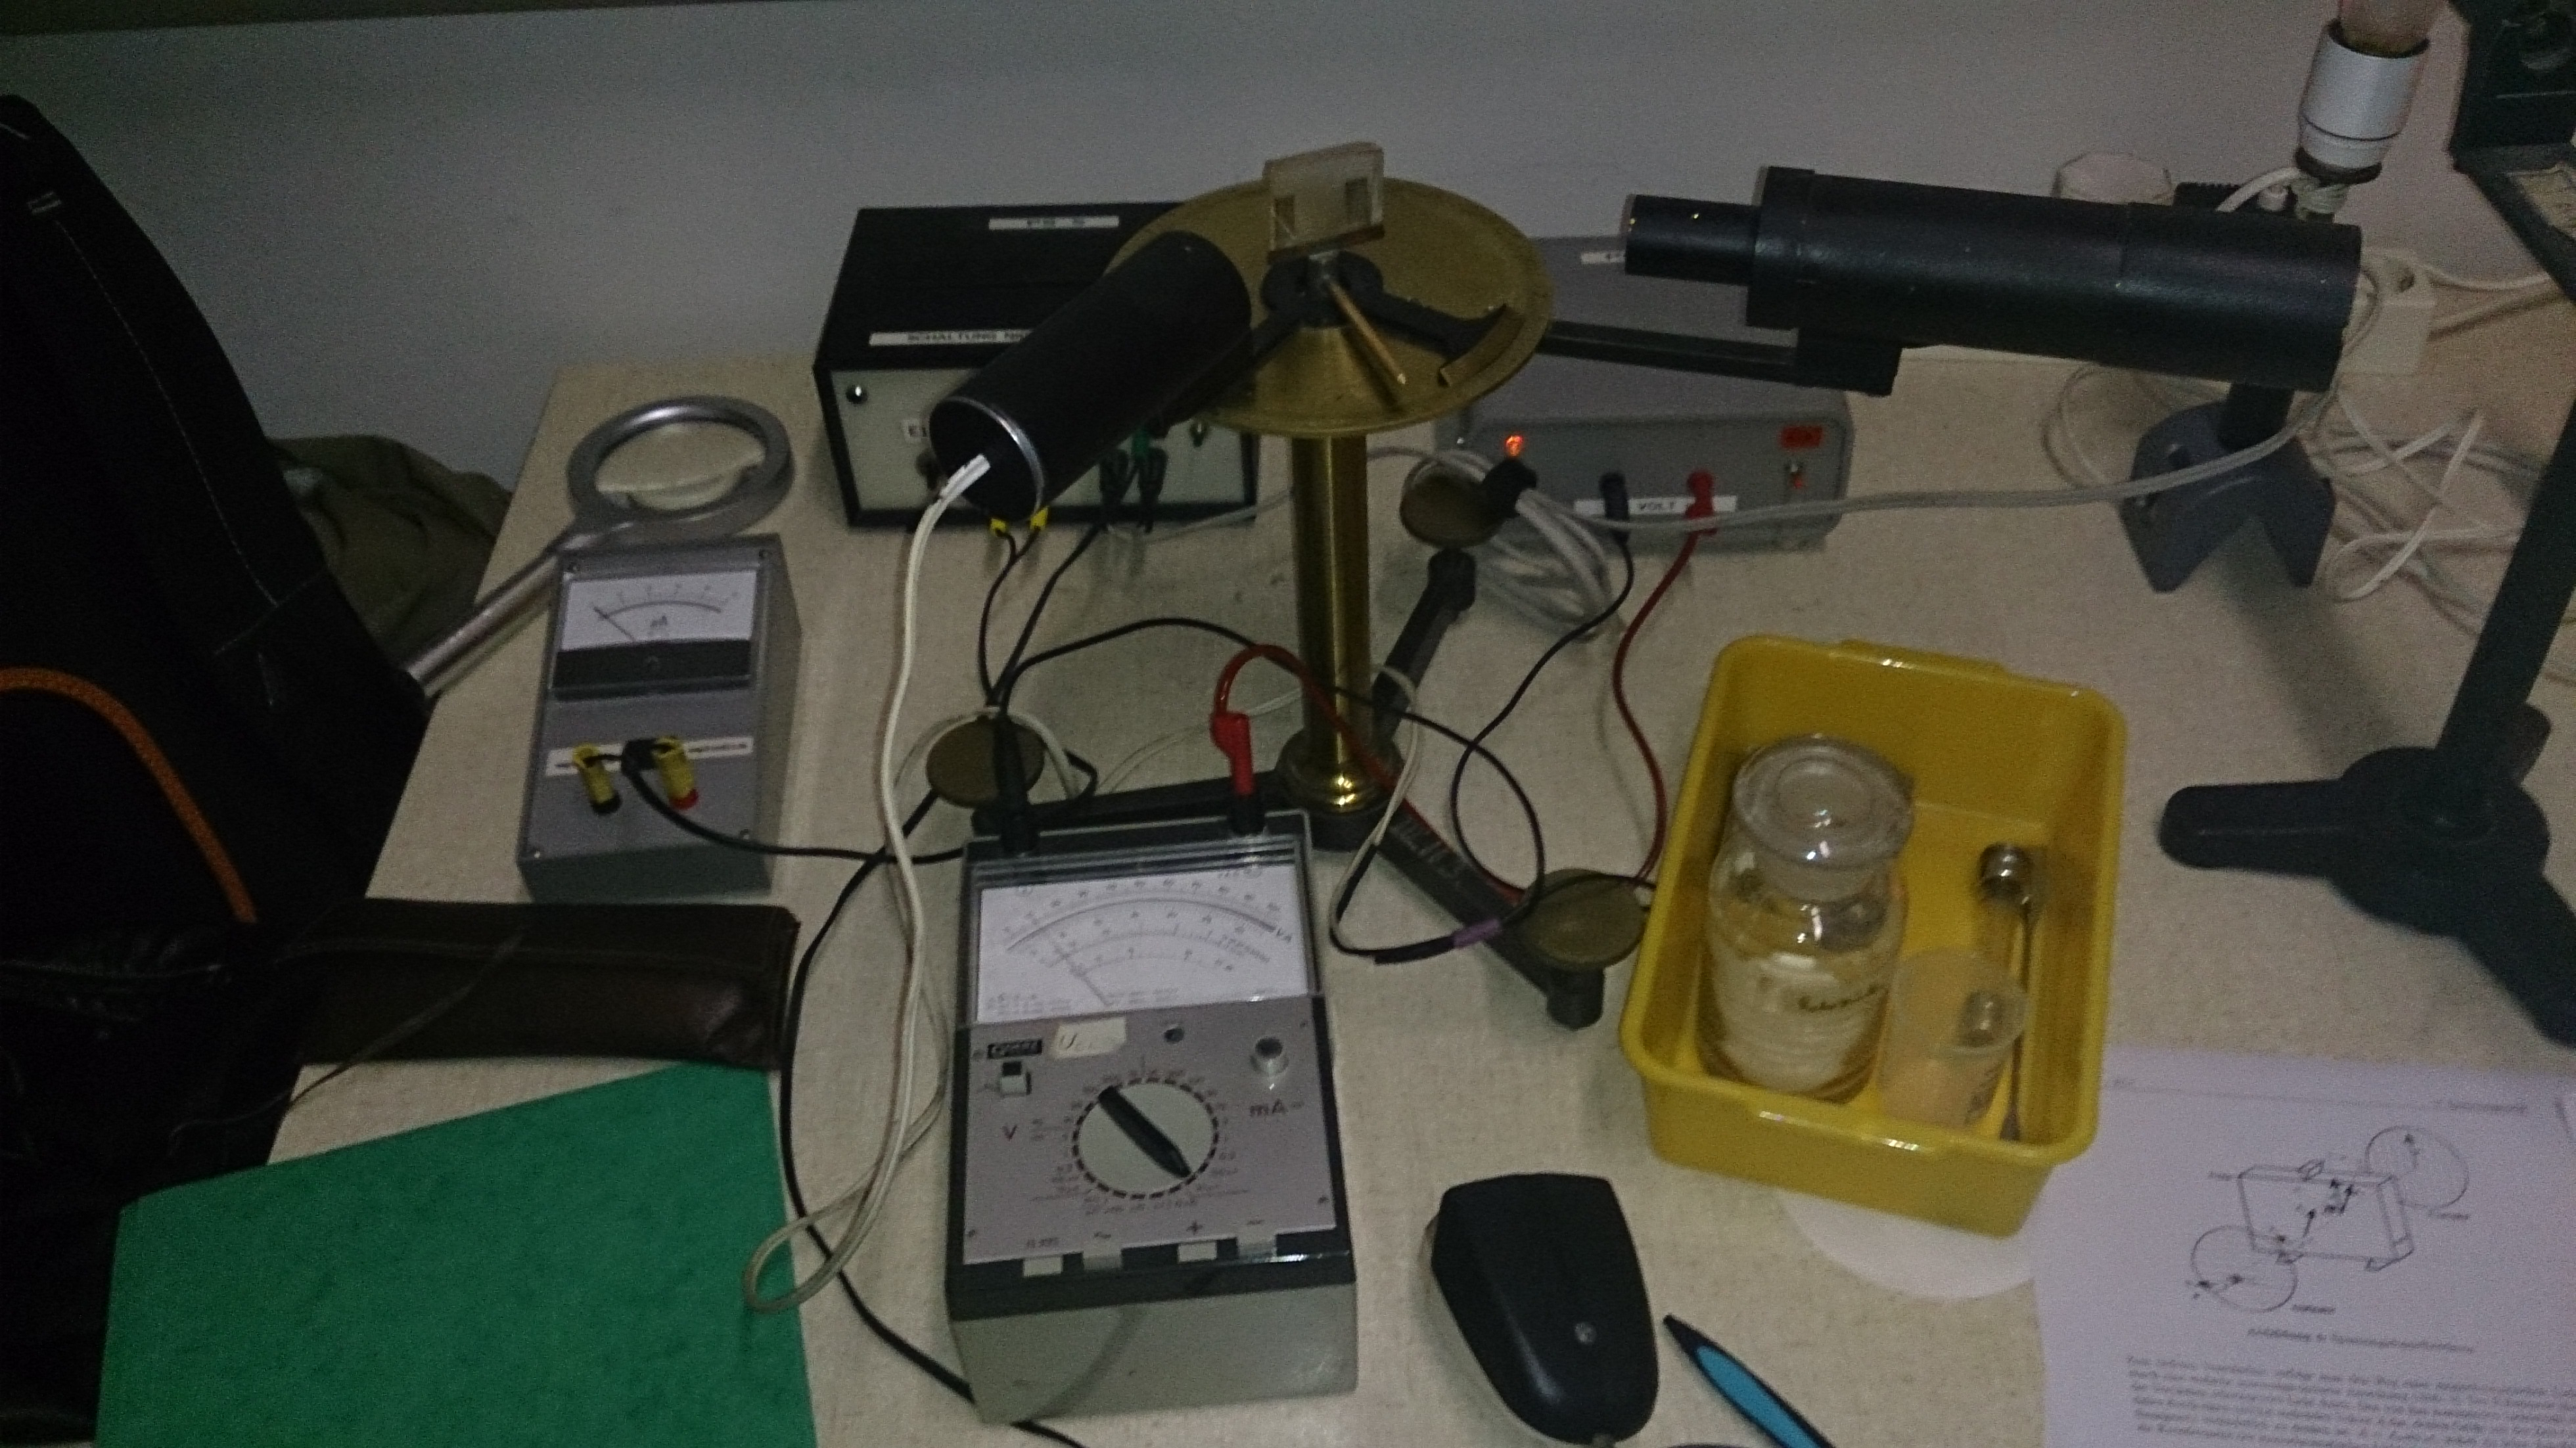
\includegraphics[scale=0.055]{./data/PS5_1_Aufbau.jpg}
	\caption{Aufbau zur Messung des Brewster-Winkel}
	\label{fig:brewster_aufbau}
\end{figure}
\noindent
Für eine kontinuierliche interpolation der Intensitätskurven wie in der Abbildung in [1](p. 3) oben, müssen für parallel und senkrecht polarisiertes Licht einige Messinge vorgenommen werden.\\
Diese Messungen werden durch neue Justierung (Abb. \ref{fig:brewster_justierung}) des Probekörpers und Ausrichtung der Diode auf das Intensitätsmaximum durchgeführt.

\begin{figure}[H]
	\centering
	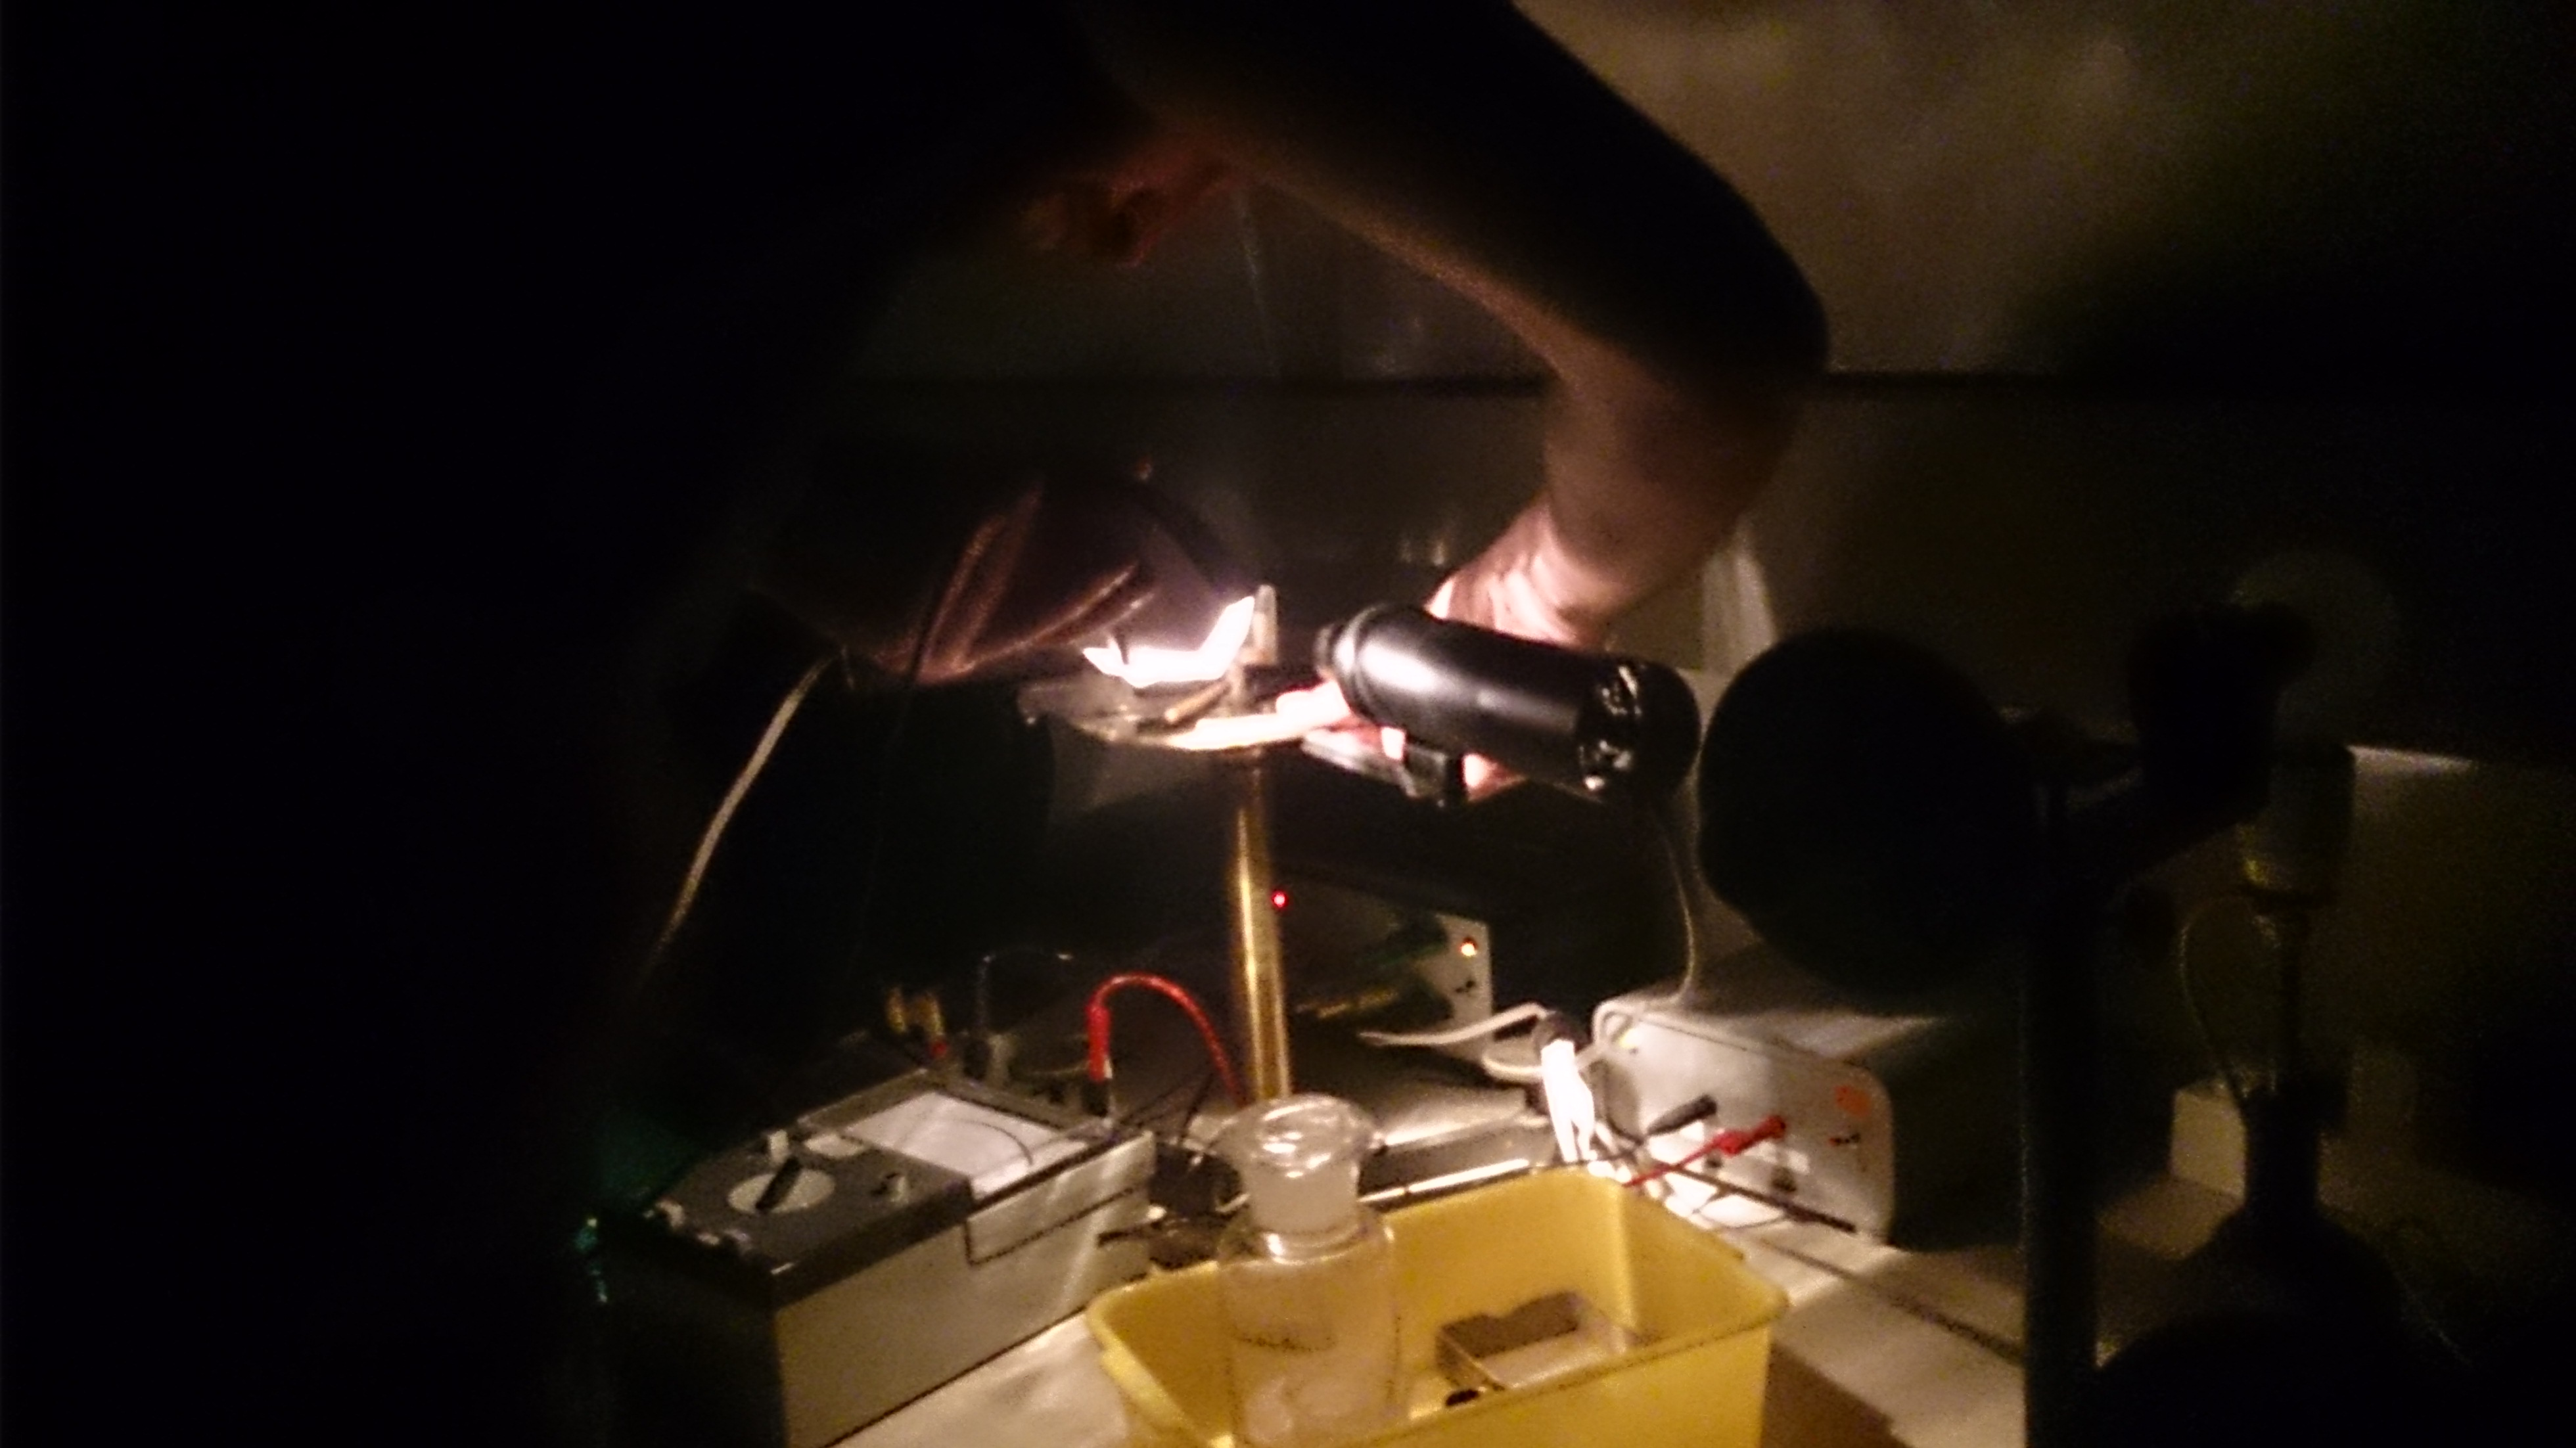
\includegraphics[scale=0.055]{./data/PS5_1_Justierung.jpg}
	\caption{Nachjustierung zur Messung des Brewster-Winkel}
	\label{fig:brewster_justierung}
\end{figure}


\subsection{Spannungsoptik}
Die Doppelbrechung tritt in anisotropen Medien auf und ruft durch z.B. Verformung oder Kompression optische Muster hervor [1](p. 6). Verwendet man weißes Licht und normal aufeinander stehende Filter (Polarisatior und Analysator, vergleiche Aufbau Abbildung \ref{fig:spannung_aufbau}) so ist nur durch das Testobjekt Licht sichtbar (Abb. \ref{fig:spannung_justierung}). Wird nun kein weißes Licht sondern Licht in einem schmalen Band verwendet, werden dunkle Linien bei Erhöhung des Drucks sichtbar.\\
Diese Linien kommen zu Stande, da durch die Verformung das polarisierte Licht doppelt (Spannungsdoppelbrechung) gebrochen wird und in Komponenten anderer Ausrichtung aufgespalten wird. Dadurch kommt es bei diesen Komponenten zu einem Gangunterschied (Bei gleichen Amplituden [1](p. 7)). Ist die Aufspaltung unter einem Winkel von 180$^\circ$ so tritt beim Analysator Auslöschung auf. Dabei ist die beherrschende Größe der Druckunterschied:

$$\delta = \frac{C}{\lambda}*d*(\sigma_1 - \sigma_2) * d$$

\noindent
wobei:\\
$\delta$ \ldots Gangunterschied\\
$\lambda$ \ldots Wellenlänge monochromatisches Licht\\
$C$ \ldots Materialkonstante\\
$\sigma_x$ \ldots Druck\\
$d$ \ldots Dicke der Probe\\

\begin{figure}[H]
	\centering
	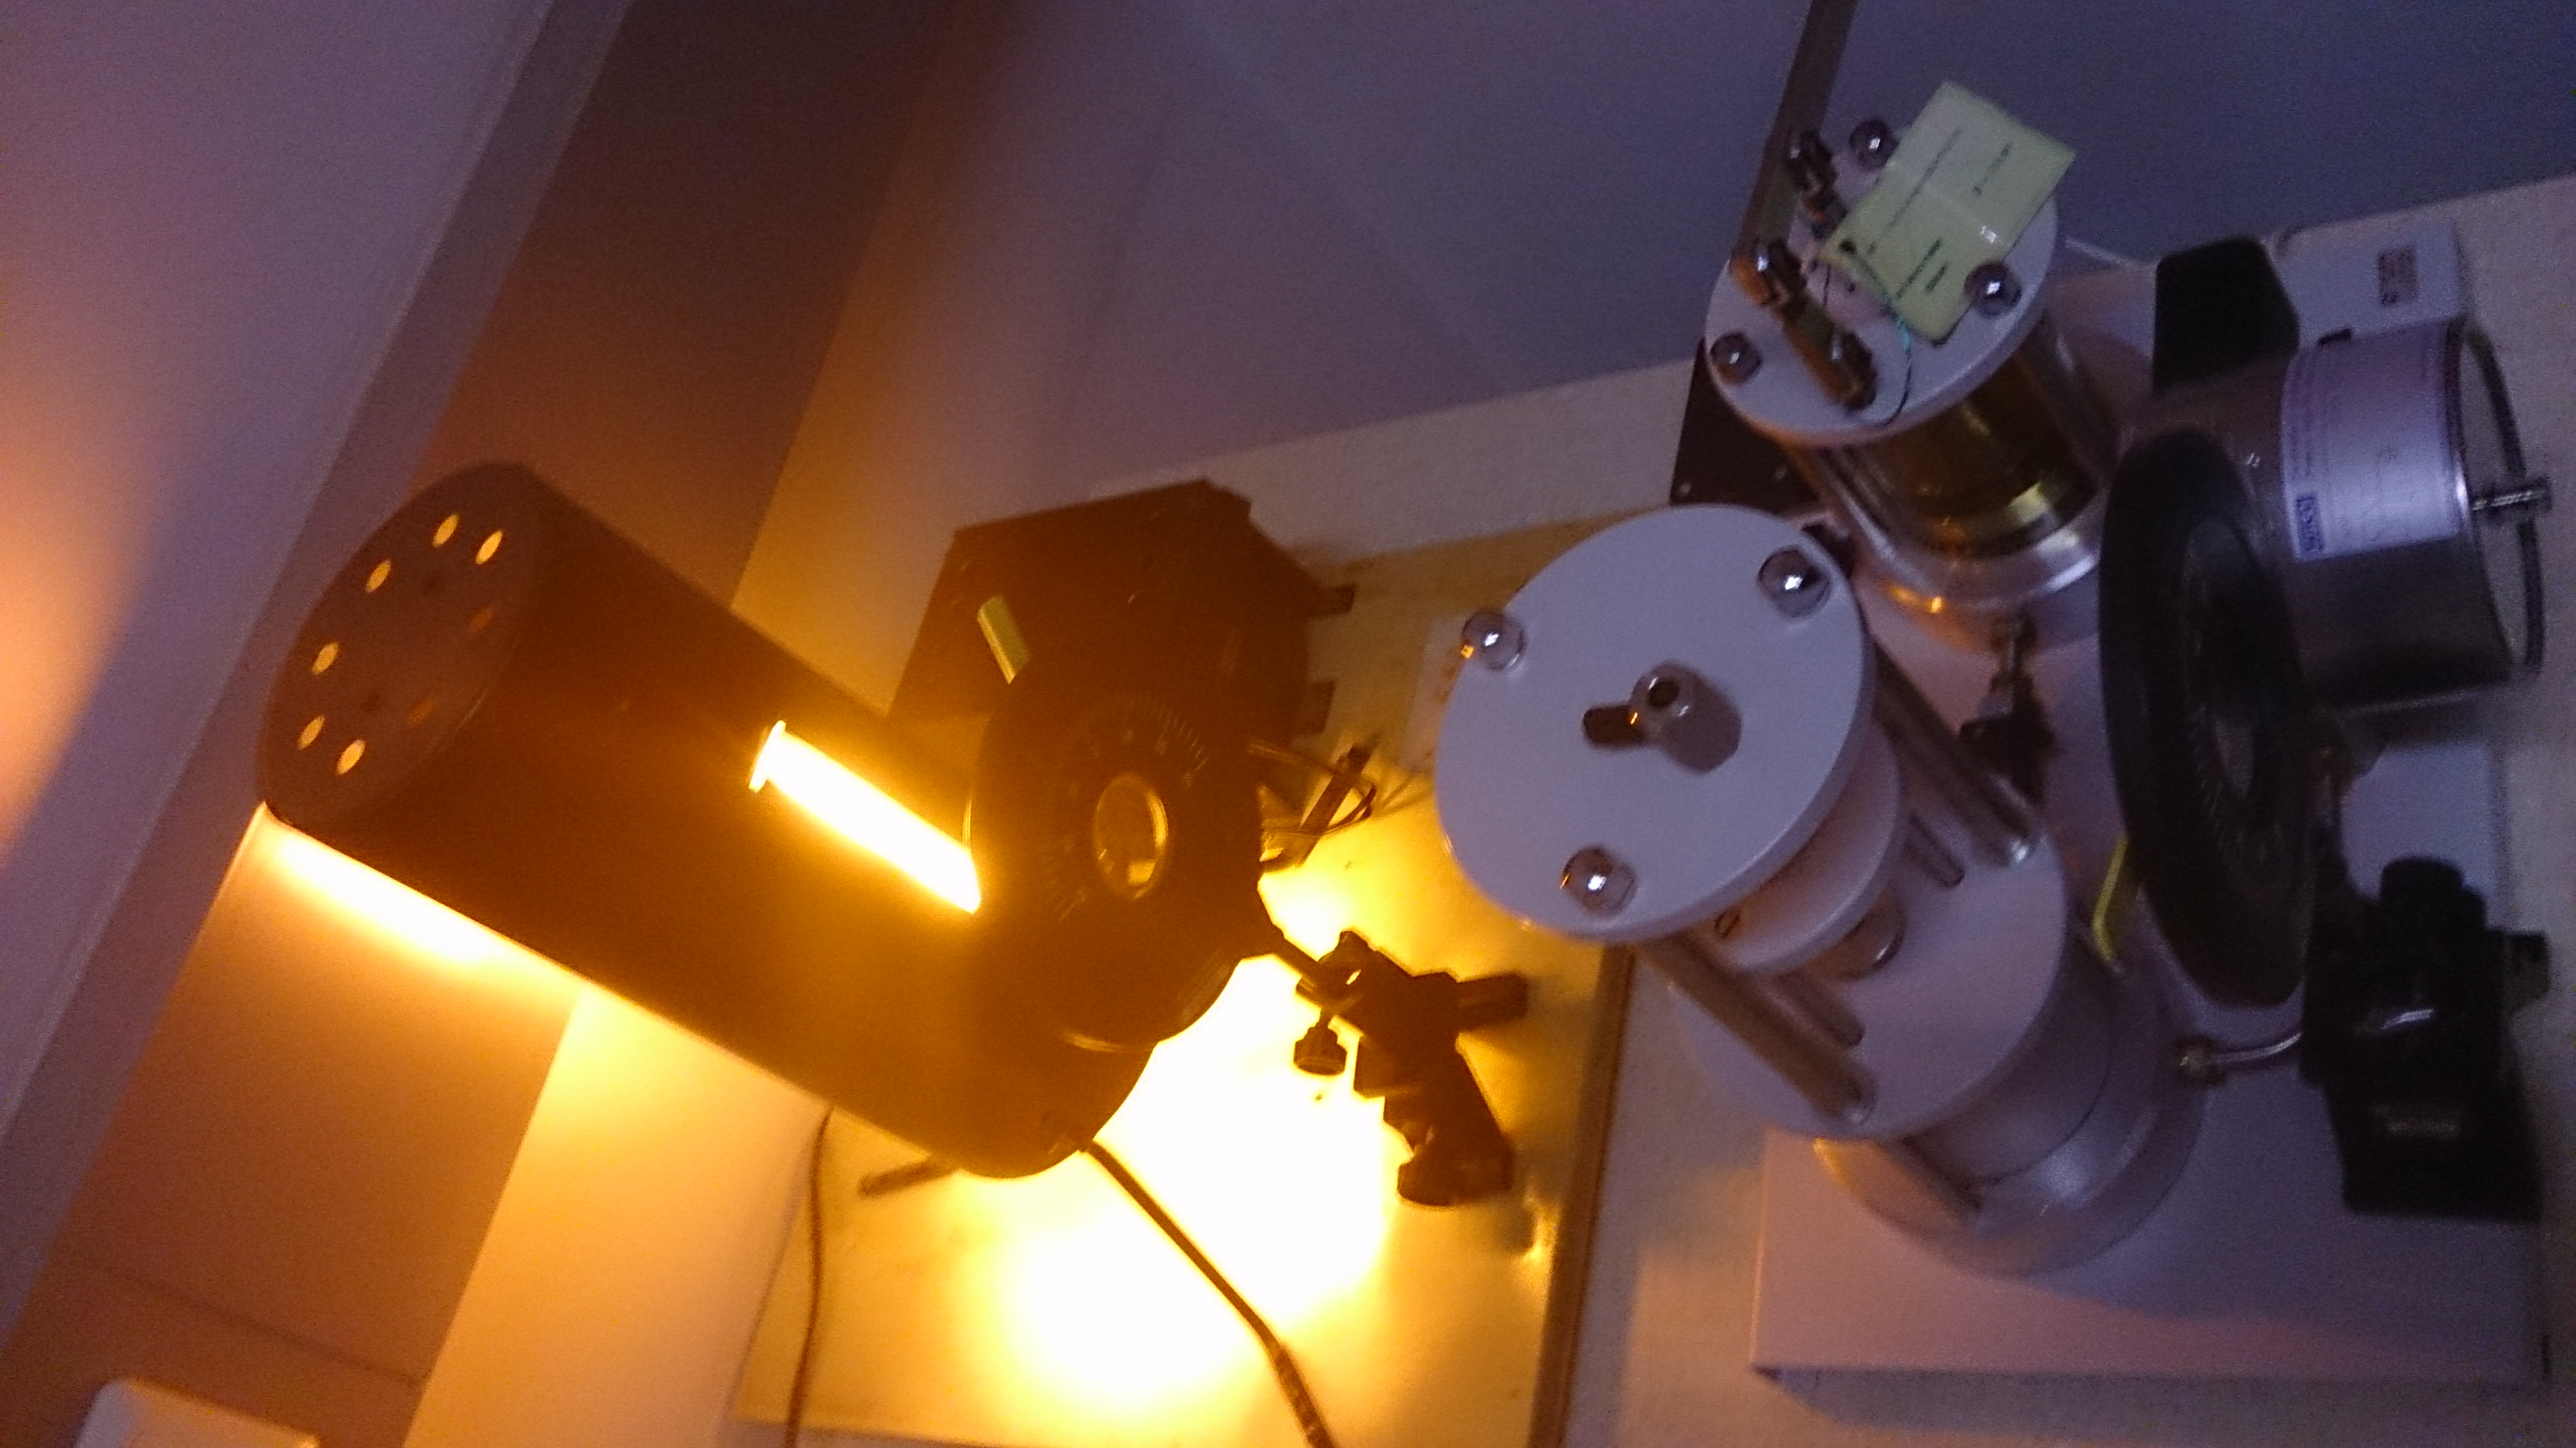
\includegraphics[scale=0.09,angle=-90]{./data/PS5_2_Aufbau.jpg}
	\caption{Aufbau zur optischen Messung einer Doppelbrechung}
	\label{fig:spannung_aufbau}
\end{figure}

\begin{figure}[H]
	\centering
	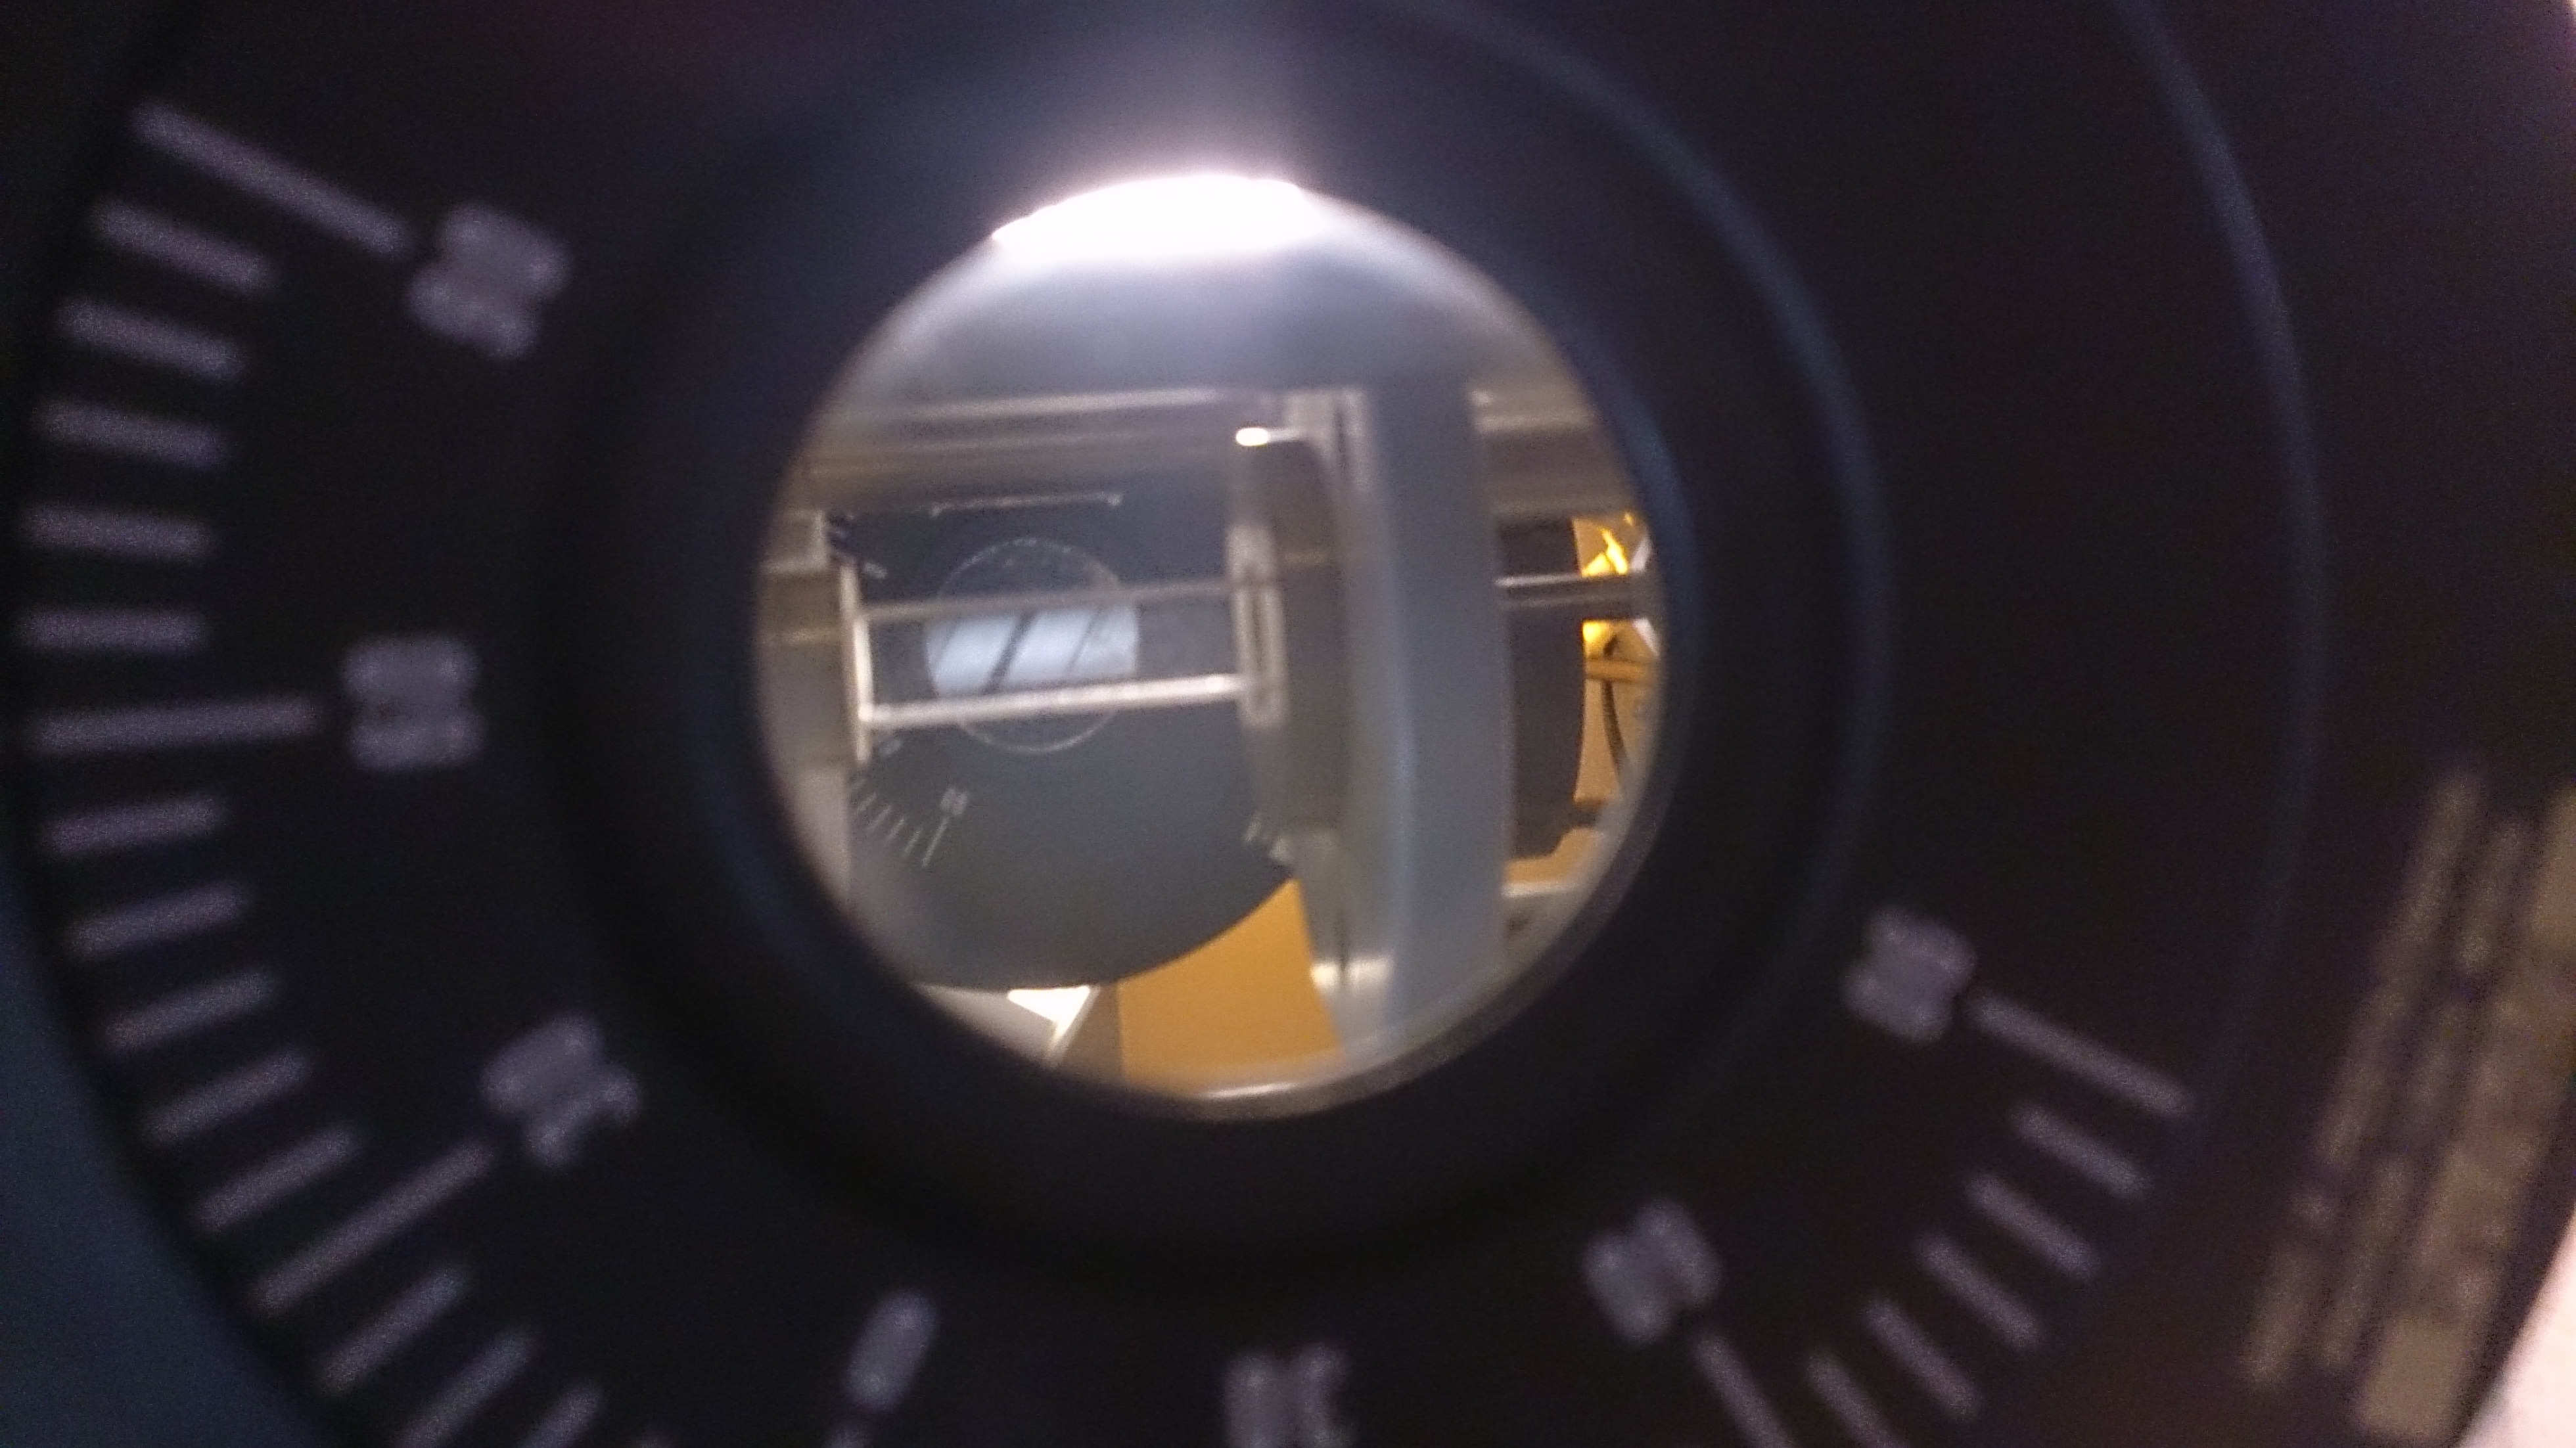
\includegraphics[scale=0.1,angle=-90]{./data/PS5_2_Filterjustierung.jpg}
	\caption{Justierung der Polarisationsfilter mit weißem Licht}
	\label{fig:spannung_justierung}
\end{figure}

\subsection{Drehung der Polarisationsebene}

In diesem Versuch wird gezeigt, dass in Quarz-Kristall sowie auch Rohrzuckerlösung die Schwingungsebene von linear polarisiertem Licht zu drehen vermögen.\\
Die Rotationsdispersion im Quarz ist darauf zurückzuführen, dass für einen außerordentlichen und einen ordentlichen Lichtstrahl, die sich in gleicher Richtung durch den Quarz bewegen, unterschiedliche Brechzahlen wirken. Dadurch ergibt sich eine Phasendifferenz und damit eine Drehung der Polarisationsebene.\\
Die Drehrichtung wird mit einem \emph{Halbschattenpolarimeter von Lippich} gezeigt: Weißes Licht gelangt durch ein erstes Prisma und wird polarisiert. Ein Hilfsprisma, nur leicht gegen den Polarisator verdreht, sorgt dafür, dass die Hälfte des Lichtes, nach einem dritten Prisma, dem Analysator, eine leicht unterschiedliche Schwingungsebene hat. Zwischen Hilfsprisma und Analysator wird die Probe (hier der Quarz) eingebracht und durch ein Fernrohr betrachtet. Dieses ist mitsamt Analysator drehbar und an einem Goniometer angebracht (in diesem Versuch geht es jedoch nur um die Drehrichtung).\\
Während das Licht durch den Quarz betrachtet wird, wird nun der Analysator in beide Richtungen gedreht, bis die richtige Farbfolge entsteht. Die Farbfolge \emph{grün - blau - rot - gelb}, die den Drehsinn anzeigt, besteht aus den Komplementärfarben derausgelöcschten Wellenlängen.\\
\\


In der Zuckerlösung wird eine eintretende Welle (linear polarisiert) in 2 entgegengesetzt rotations-polarisierte Wellen aufgespaltet. Diese gleichen sich zwar in ihrer Frequenz und Amplitude (also der halben Amplitude der eintretenden Welle), haben jedoch eine verschiedene Phasengeschwindigkeit.\\
Durch diese unterschiedlichen Ausbreitungsgeschwindigkeiten, tritt wieder ein linear polarisierter Strahl aus der Zuckerlösung aus, jedoch ist die Polarisationsebene gedreht, abhängig von der Weglänge in der Lösung.\\
Gemessen wird mit einem \emph{Polarimeter nach Mitscherlich}. Das Prinzip ist ähnlich dem des Halbschattenpolarimeters aus der Quarzmessung. Als Lichtquelle wird eine Natriumdampflampe verwendet mit Wellenlänge $\lambda = 590$ nm. Die Küvette mit der Zuckerlösung wird in einem geschlossenen Schacht im Strahl gehalten.\\
Zuerst wird ohne Zuckerlösung der 0-Punkt bestimmt, an dem sich die Polarisationsrichtung umkehrt. Danach wird, mit eingelegter Lösung, der Umkehrpunkt bestimmt und daraus der Winkel, um den die Polarisationsebene gedreht wurde.
Die gesuchte \emph{spezifische Drehung} $[\alpha]$ der Lösung ist gegeben durch
$$[\alpha] = \frac{\alpha}{C \cdot l}$$
mit gemessenem Drehwinkel $\alpha$, Küvettenlänge $l$ und Lösungskonzentration $C$.



%TODO Bild aus Anleitung oder so

%%%%%%%%%%%%%%%%%%%%%%%%%%%%%%%%%%%%%%%%%%%%%%%%
%%%%%%%%%%%%%%%%%%%%%%%%%%%%%%%%%%%%%%%%%%%%%%%%
\section{Resultate}

\subsection{Brewster Winkel}
\textbf{Senkrecht Polarisiert}\\
Bei $180^\circ$ (nicht exakt, da Detektor nicht im Zentrum des Gehäuses) gibt es ein Maximum der Intensität mit \textbf{(0.94 $\pm$ 0.005)mA}.\\

\begin{figure}[H]
	\centering
	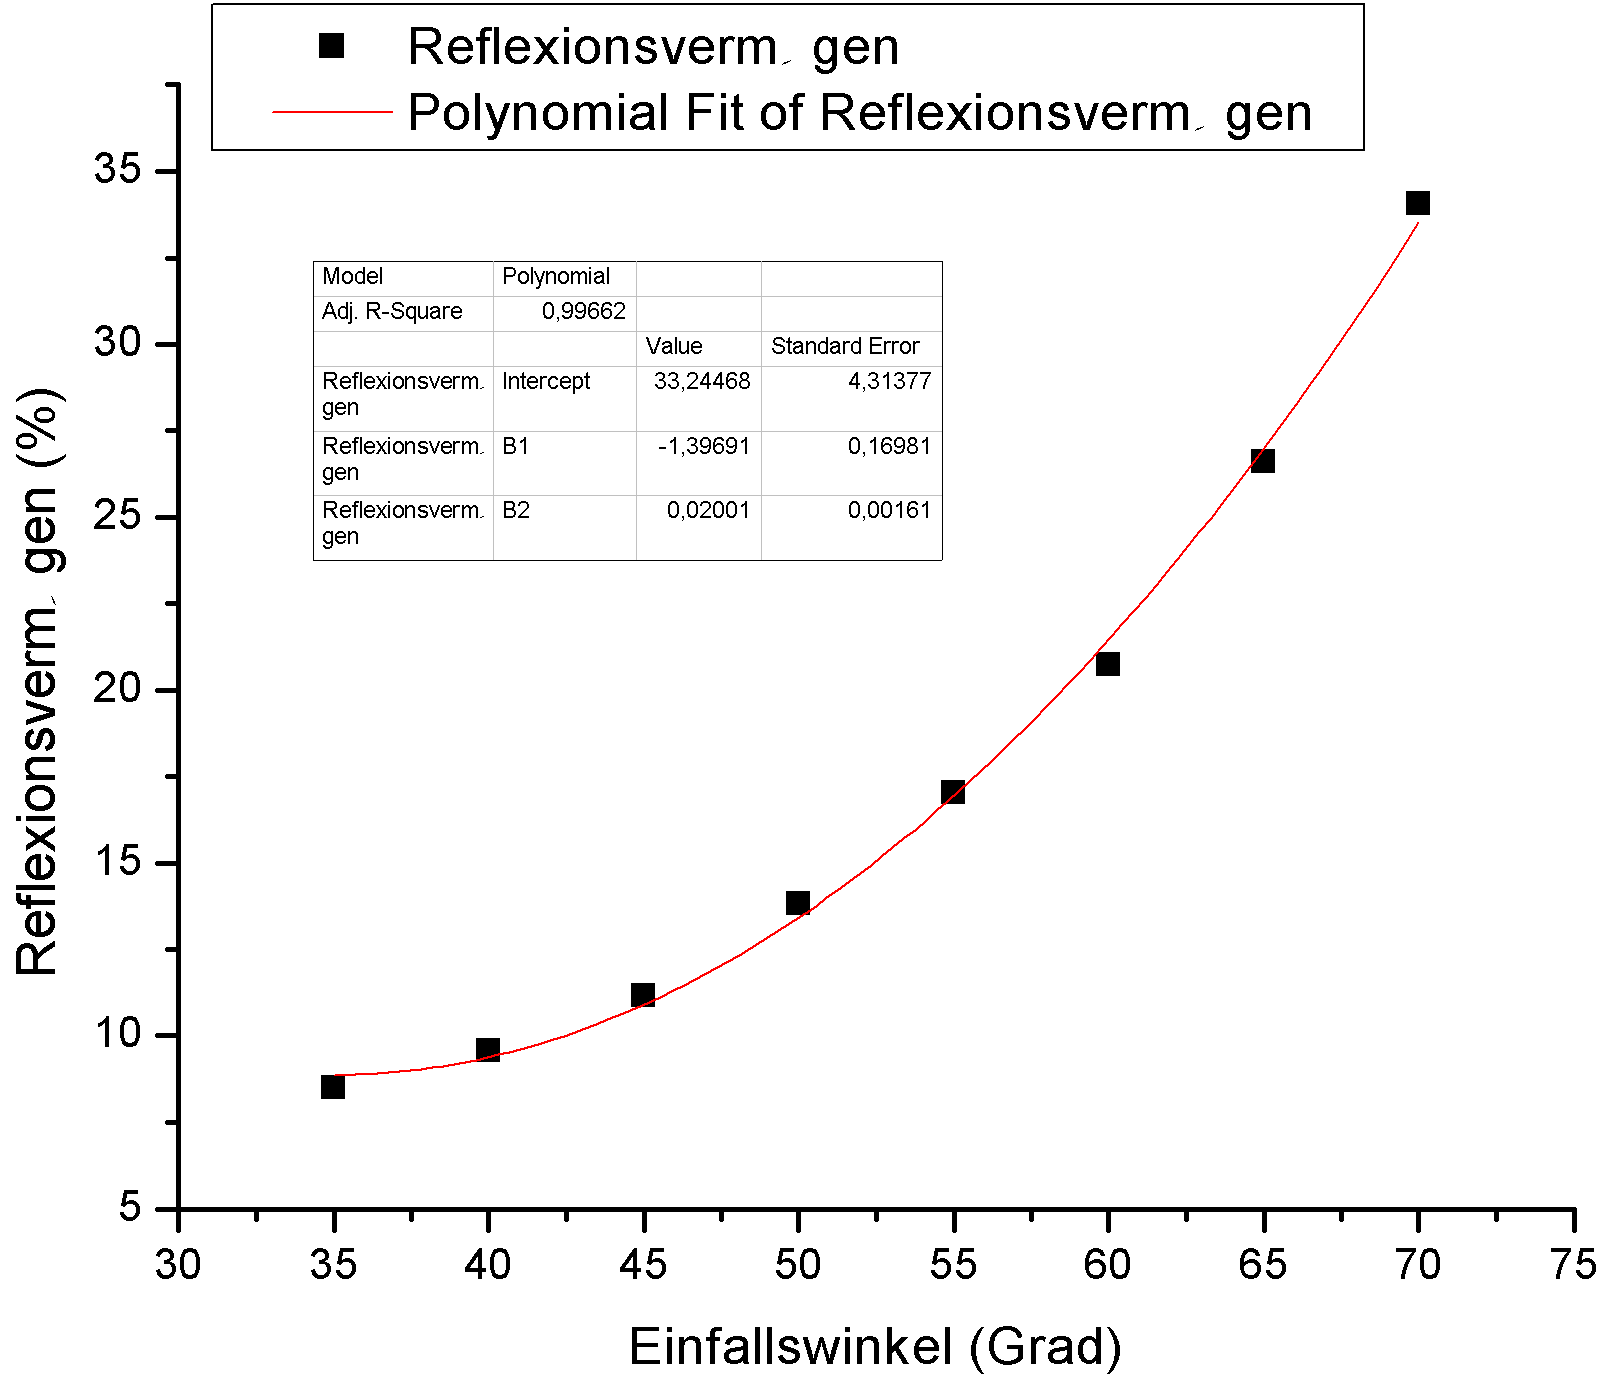
\includegraphics[scale=0.28]{./data/R_S_Plot.png}
	\caption{Reflexionsvermögen senkrecht polarisiertes Licht mit polynomiellem Fit}
	\label{fig:r_s_plot}
\end{figure}

\begin{figure}[H]
	\centering
	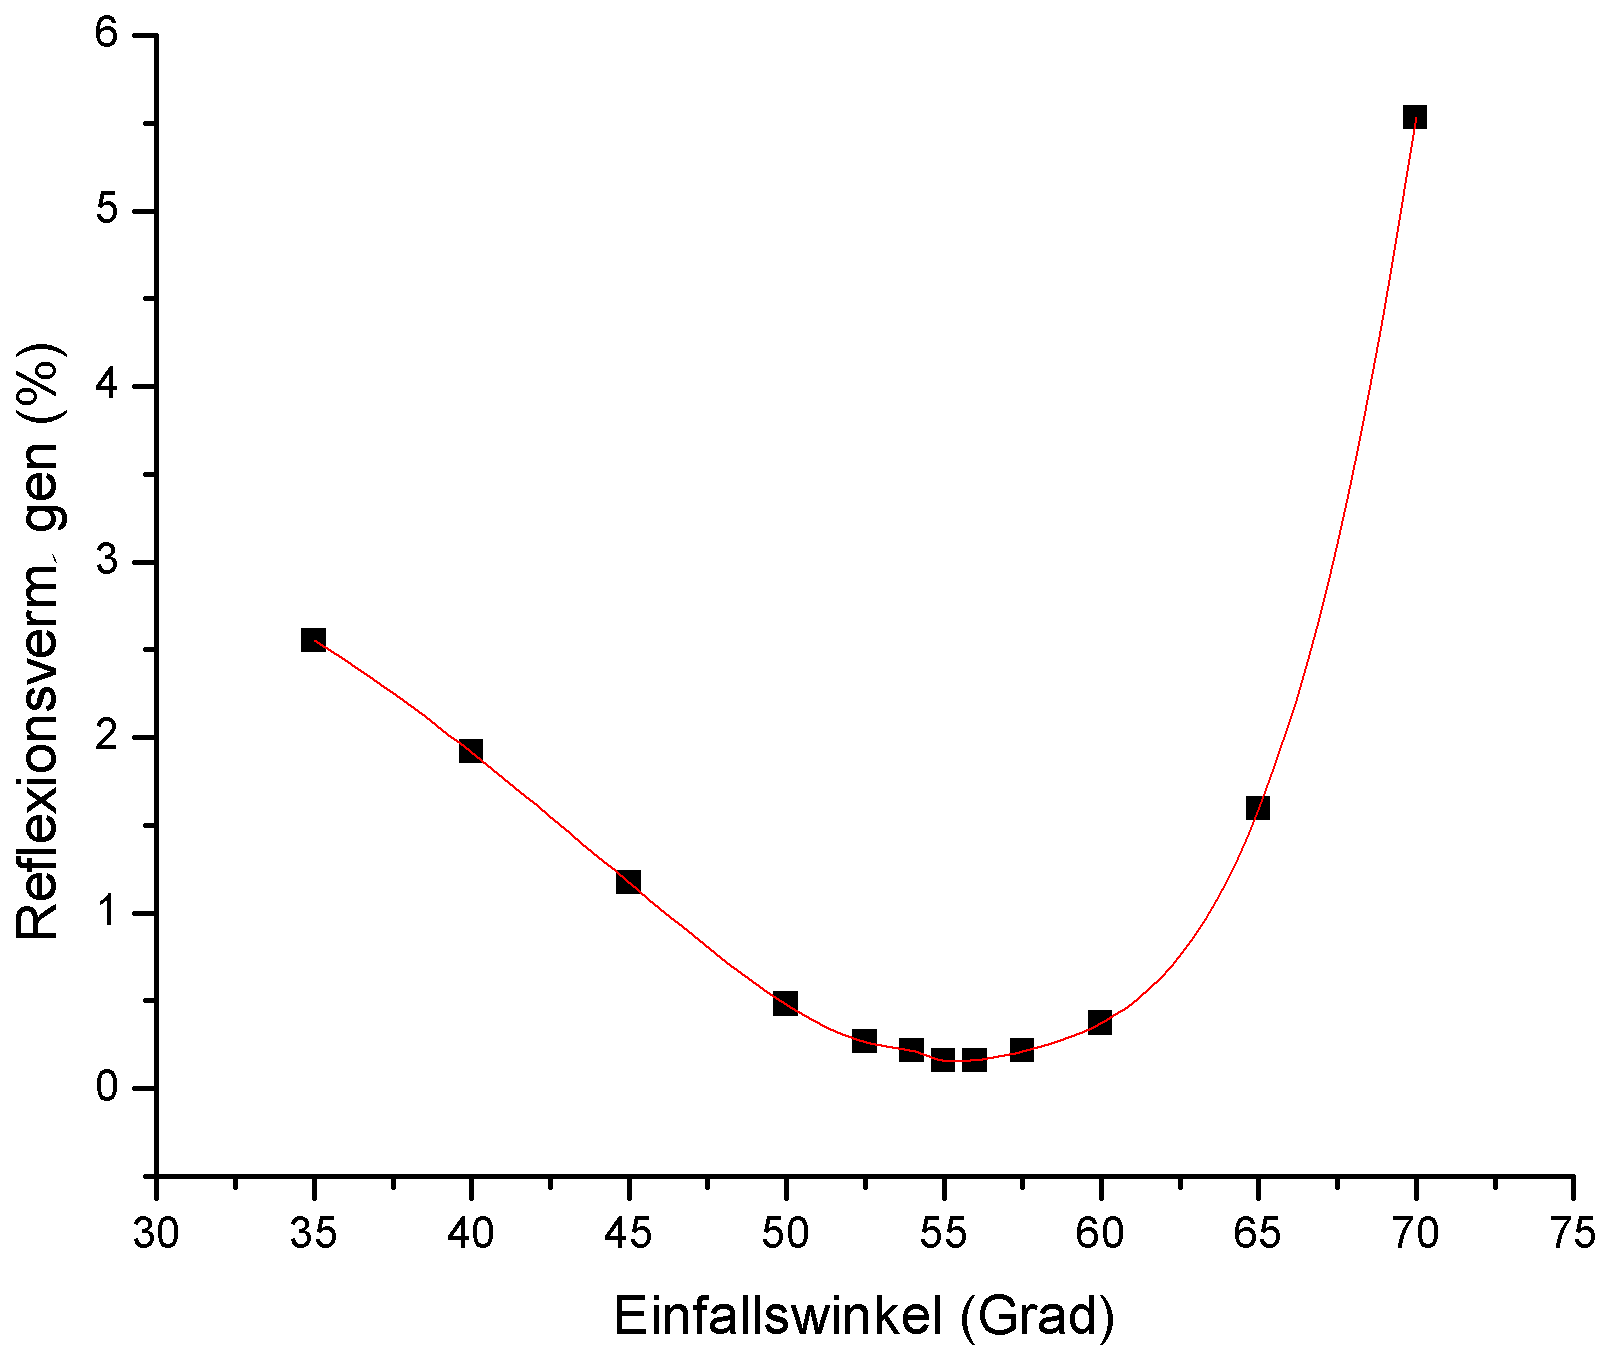
\includegraphics[scale=0.28]{./data/R_P_Plot.png}
	\caption{Reflexionsvermögen parallel polarisiertes Licht mit Interpolation}
	\label{fig:r_p_plot}
\end{figure}
In Abbildung \ref{fig:r_p_plot} ein Winkel von (55 $\pm$ 5)$^\circ$ als Brewster-Winkel ersichtlich.
\subsection{Spannungsoptik}




\subsection{Drehung der Polarisationsebene}

\textbf{Quarz:}\\
Die Drehrichtung des Quarzes ist \emph{gegen den Uhrzeigersinn.} \\
Getestet wurden alle 3 verfügbaren Steine, die Farbfolge ist deutlich zu sehen.\\
\\
\textbf{Rohrzuckerlösung:}\\
$l=(1.909\pm 0.001)dm$\\
$C = (10.00 \pm 0.41)\%$\\
$\alpha = (13.3 \pm 0.2)^\circ$
$$[\alpha] = (69.7 \pm 3.1)$$

(Literaturwert aus Bergmann-Schaefer; Lehrbuch der Experimentalphysik, Bd. 3: Optik; p. 538: \textbf{66.5})

%%%%%%%%%%%%%%%%%%%%%%%%%%%%%%%%%%%%%%%%%%%%%%%%
%%%%%%%%%%%%%%%%%%%%%%%%%%%%%%%%%%%%%%%%%%%%%%%%
\section{Diskussion}

\subsection{Brewster Winkel}
Da wir mit einem Amperemeter den Strom gemessen haben und beim Brewster Winkel kein Strom feststellbar war, wurde wohl im Anleitungstext ein Fotowiderstand (kein Strom fließt) und eine Fotodiode [3] (Strom fließt bei Einstrahlung) vertauscht. \\
Die Resultate zeigen eindeutig das bei parallel polarisiertem Licht keine Reflexion stattfindet  (Abb. \ref{fig:r_p_plot}) bei senkrecht polarisiertem Licht jedoch Totalreflexion (Abb. \ref{fig:r_s_plot}). \\
Der Brewster-Winkel konnte leider nur auf einige Grad genau bestimmt werden, da im zutreffenden Bereich nur noch um 1 $\mu$A messbar war, welches aber auch vom Hintergrund (Wärme, Licht von außen etc.) verursacht werden konnte. Bei einem solch kleinem Strom könnte sogar Induktion vom Netzteil die Ursache sein.


\subsection{Spannungsoptik}




\subsection{Drehung der Polarisationsebene}




\section{Quellen}
$[1]$ Anleitung, \url{http://www.univie.ac.at/anfpra/neu1/ps/ps5/PS5.pdf}\\
$[2]$ Fotowiderstand \url{https://de.wikipedia.org/wiki/Fotowiderstand}\\
$[3]$ Fotodiode \url{https://de.wikipedia.org/wiki/Fotodiode}\\
\end{multicols}

\end{document}